\label{sec:problem_description}
Given the workpiece geometry and the available fixture types and quantities, the objective is to determine which fixtures should be selected and their placement so as to maximize workpiece stability during machining.

To ensure the feasibility of a placement, the following constraints must be satisfied:
\begin{enumerate}
	\item the number of fixtures placed for each type must not exceed the number available;
	\item fixtures must be placed so as to satisfy the specified minimum horizontal and vertical safety distances;
	\item fixtures must be positioned within the workpiece boundaries and beneath its surface;
	\item fixtures must not overlap each other;
	\item fixtures must not be located beneath areas to be extruded, to prevent damage.
\end{enumerate}

To illustrate the constraints, Figure~\ref{fig:constraints_axample} shows examples of valid and invalid fixture placements. Fixture $F_6$ is invalid because it violates the minimum horizontal safety distance with respect to fixtures $F_3$ and $F_4$, whereas fixture $F_5$ is invalid because it is positioned beneath an area to be extruded.

\begin{figure}[t]
	\centering
	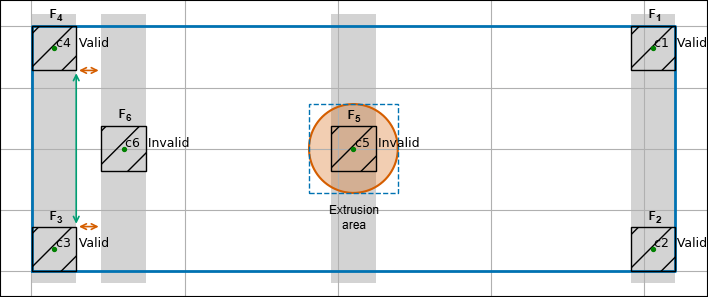
\includegraphics[width=0.65\linewidth]{img/valid_invalid_positions_example.png}
	\caption{Example of valid and invalid fixture placements. For a fixture placement to be valid, the fixture must lie within the workpiece boundaries, satisfy the required safety distances from the other fixtures, and not be positioned beneath an area to be extruded.}
	\label{fig:constraints_axample}
\end{figure}

The formulation of these constraints depends on the chosen solution strategy and the corresponding decision variables and is therefore presented separately for each of the considered solution techniques. All approaches, however, are defined over the same set of input parameters listed below:
\begin{itemize}
	\item the width $\wtab$ and height $\htab$ of the machine worktable;
	\item the minimum horizontal distance $\wmin$ between two fixtures placed on different bars;
	\item the minimum vertical distance $\hmin$ between two fixtures placed on the same bar;
	\item the number $\ntypes$ of different fixture types;
	\item the number $\nfix_i$ of available fixtures for each type $i \in [1..\ntypes]$;
	\item the total number of available fixtures $\nfix = \sum_{i=1}^{\ntypes} \nfix_i$;
	\item the minimum $\nmin$ and maximum $\nmax$ number of fixtures to place;
	\item the width $\wfix_i$ and height $\hfix_i$ of each fixture of type $i$;
	\item the workpiece shape, represented by a set of linear inequalities of the form $\mathtt{a}x + \mathtt{b}y + \mathtt{c} \leq 0$;
	\item the number $\numext$ of areas to be extruded;
	\item the width $\ewside_i$, height $\ehside_i$, and the coordinates $(\xext_i,\yext_i)$ of the lower-left corner of the smallest axis-aligned rectangle enclosing each extrusion area $i \in [1..\numext]$.
\end{itemize}

Extrusion areas are typically represented by simple geometric shapes, such as circles, rectangles, or ellipses, whereas more complex geometries are refined manually. To facilitate the solution process, each extrusion area is approximated by its smallest enclosing rectangle (as illustrated in Figure~\ref{fig:constraints_axample}), which is represented by the coordinates of its lower-left corner together with its width and height.

To evaluate the quality of a fixture layout, two objective functions are considered. The CP and MIP models optimize the objective function $\fdist$ proposed in~\cite{vitali2026constraint}, which maximizes the sum of the pairwise Manhattan distances between fixture centroids, augmented by the total area of the selected fixtures:

\begin{equation}
	\fdist = \sum_{1 \le i < j \le n} \left(|cx_i - cx_j| + |cy_i - cy_j|\right) + \sum_{k=1}^{n} (\wfix_{t_k} \cdot \hfix_{t_k})
	\label{eq:f_dist}
\end{equation}

where $(x_k,y_k)$ are the coordinates of the lower-left corner of the $k$-th placed fixture, having type $t_k$ ($n$ is the total number of placed fixtures), and centroid $(cx_k,cy_k)=\left(x_k+\frac{\wfix_{t_k}}{2},,y_k+\frac{\hfix_{t_k}}{2}\right)$.

The use of the $\fdist$ objective function for the CP and MIP models is motivated by the fact that computing the principal moment of inertia expressed in Eq.~\ref{eq:finer} involves nonlinear operations, including squaring, square roots, and transcendental functions (sine and cosine), which substantially increase the computational effort required by CP and MIP solvers~\cite{leyffer2009applications}.

The Q-learning algorithm, on the other hand, is not affected by the nonlinear computations required to evaluate $\finer$ and therefore directly incorporates the moments of inertia into its reward function, as described in Section~\ref{sec:rl_algorithm}.

The CP model, the MIP model, and the Q-learning algorithm are used to generate initial feasible layouts. For each instance, the best layout produced by these methods is then refined using the PSO algorithm described in Section~\ref{sec:pso_algorithm}, which optimizes $\finer$ while introducing the fixture rotation angle as an additional decision variable.